\documentclass[class=minimal,border=5pt]{standalone}
\usepackage{ufcd}
\usepackage{bm}
\usepackage{booktabs}
\usepackage{color}

\usepackage{tikz}
\usepackage{tikz-qtree}
\usetikzlibrary{fit}
\usetikzlibrary{trees}
\usetikzlibrary{shapes.geometric}
\usetikzlibrary{mindmap,backgrounds}
\usetikzlibrary{positioning,shapes,shadows,arrows,calc}
\pgfdeclarelayer{background}
\pgfdeclarelayer{foreground}
\pgfsetlayers{background,main,foreground}

\tikzstyle{data}=[rectangle, draw=black, rounded corners, text centered, text width=8em, fill=white, drop shadow]
\tikzstyle{core}=[rectangle, draw=black, text centered, fill=black!10, text width=8em, drop shadow]
\tikzstyle{myarrow}=[->, thick]

\definecolor{light_red}{RGB}{222,56,49}

\begin{document}
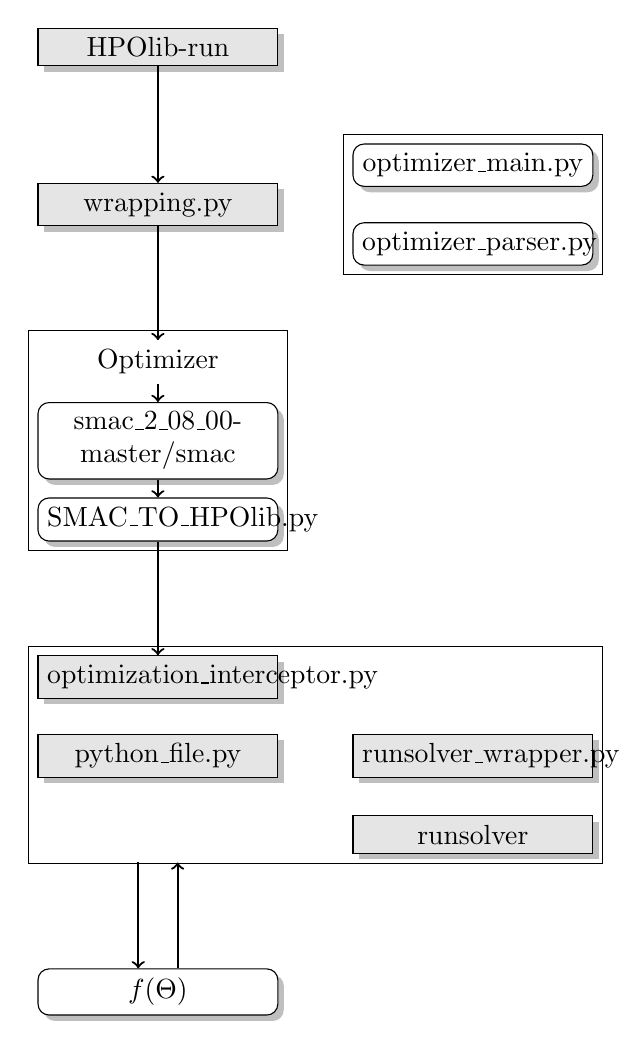
\begin{tikzpicture}[node distance=2cm]
        \node (HPOlib-run) [core] {HPOlib-run};
        \node (wrapping) [core, below of=HPOlib-run] {wrapping.py};
        \node (optimizer_main) [data, right of=wrapping, node distance=4cm, yshift=0.5cm] {optimizer\_main.py};
        \node (optimizer_parser) [data, right of=wrapping, node distance=4cm, yshift=-0.5cm] {optimizer\_parser.py};
        
        \node [draw=black, fit={(optimizer_main) (optimizer_parser)}] {};
        
        % Optimizer
        \node (optimizer) [below of=wrapping] {Optimizer};
        \node (SMAC) [data, below of=optimizer, node distance=1cm] {smac\_2\_08\_00-master/smac};
        \node (SMAC_TO_HPOlib) [data, below of=SMAC, node distance=1cm] {SMAC\_TO\_HPOlib.py};
        
        \node [draw=black, fit={(SMAC) (SMAC_TO_HPOlib) (optimizer)}] {};
        
        % Target Function evaluation
        \node (optimization_interceptor) [core, below of=SMAC_TO_HPOlib] {optimization\_interceptor.py};
        
        \node (python_file) [core, below of=optimization_interceptor, node distance=1cm] {python\_file.py};
        \node (runsolver_wrapper) [core, right of=python_file, node distance=4cm] {runsolver\_wrapper.py};
        %\node (mysqldbtae) [core, right of=runsolver_wrapper, node distance=4cm] {mysqldbtae.py};
        \node (runsolver) [core, below of=runsolver_wrapper, node distance=1cm] {runsolver};
        
        \node [draw=black, fit={(optimization_interceptor) (python_file) (runsolver_wrapper) (runsolver)}] {};
        
        % Target Function
        \node (function) [data, below of=optimization_interceptor, node distance=4cm] {$f(\Theta)$};

        \draw[myarrow] (HPOlib-run) -- ($(wrapping.north)+(0,0)$);
        \draw[myarrow] (wrapping) -- ($(optimizer.north)+(0,0)$);
        \draw[myarrow] (optimizer.south) -- ($(SMAC.north)+(0,0)$);
        \draw[myarrow] (SMAC.south) -- ($(SMAC_TO_HPOlib.north)+(0,0)$);
        \draw[myarrow] (SMAC_TO_HPOlib.south) -- ($(optimization_interceptor.north)+(0,0)$);
        
        \draw[myarrow] ($(optimization_interceptor.south)-(0.25,2.08)$) -- ($(function.north)-(0.25,0)$);
        \draw[myarrow] ($(function.north)+(0.25,0)$) -- ($(optimization_interceptor.south)+(0.25,-2.08)$);


        %\begin{pgfonlayer}{background}

        % Configuration Process
        %\path (optimizer_parser -| optimizer_parser.west)+(-0.25,1.25) node (resUL) {};
        %\path (optimization_interceptor.east |- optimization_interceptor.south)+(2.25,-1.0) node(resBR) {};
        %\path [rounded corners, draw=black!50, dashed] (resUL) rectangle (resBR);
        %        \path (optimization_interceptor.east |- optimization_interceptor.south)+(-1.4,-0.8) node [text=black!60] {SMBO};

	%\end{pgfonlayer}

\end{tikzpicture}

\end{document}
